\PassOptionsToPackage{table}{xcolor}
\documentclass[aspectratio=169,xcolor=dvipsnames,11pt]{beamer}
\usetheme{SimplePlusAIC}
\usepackage{amsmath}
\usepackage{animate}
\usepackage{hyperref}
\usepackage{cleveref}
\usepackage{caption}
\usepackage{graphicx} % Allows including images
%\usepackage{subfig}
\usepackage{subcaption}
\usepackage{booktabs} % Allows the use of \toprule, \midrule and  \bottomrule in tables
\usepackage{svg} %allows using svg figures
\usepackage{tikz}
\usetikzlibrary{intersections}
\usetikzlibrary{arrows.meta, calc, quotes, tikzmark}
\usepackage{makecell}
\usepackage{multirow}
\usepackage{appendixnumberbeamer}
\usepackage{wrapfig}
\usepackage{verbatim}
\usepackage{tcolorbox}
\usepackage{multicol}
\setlength{\columnsep}{1cm}
%\usepackage[dvipsnames]{xcolor}

\usepackage{hhline}
\usepackage{relsize}
\usepackage{bm}
%Select the Epilogue font (requires luaLatex or XeLaTex compilers)
%\setsansfont{Epilogue}[
  %  Path=./epilogueFont/,
  %  Scale=0.9,
  %  Extension = .ttf,
   % UprightFont=*-Regular,
   % BoldFont=*-Bold,
   % ItalicFont=*-Italic,
    %BoldItalicFont=*-BoldItalic
    %]
    \usefonttheme[onlymath]{serif}
% \usepackage{ eulervm } % Euler VM as math serif font

\newcommand*{\defeq}{\stackrel{\text{def}}{=}}
\newcommand{\grad}{\nabla}
\newcommand{\lap}{\Delta}
\newcommand{\weaklyto}{\rightharpoonup}
\newcommand{\weakstar}{\stackrel{*}\rightharpoonup}
\newcommand{\cts}{\hookrightarrow}
\newcommand{\ctsDense}{\xhookrightarrow{d}}
\newcommand{\ctsCompact}{\xhookrightarrow{c}}
\newcommand{\E}{\mathbb{E}}
\newcommand{\pP}{\mathbb{P}}
\newcommand{\R}{\mathbb{R}}
\newcommand{\ER}{\overline{\mathbb{R}}}
\newcommand{\cR}{\mathcal{R}}
\newcommand{\cJ}{\mathcal{J}}
\newcommand{\cG}{\mathcal{G}}
\newcommand{\CVaR}{\textup{CVaR}}
\newcommand{\D}{\textup{ d}}
\newcommand{\dd}{\mathrm{d}}
\newcommand{\fa}{\text{for all }}
\DeclareMathOperator*{\essinf}{\vphantom{p}ess\,inf}
\DeclareMathOperator{\sigmoid}{expit} % a.k.a. logistic sigmoid

\usepackage[ruled,vlined,algo2e]{algorithm2e}
\crefname{algocf}{algorithm}{algorithms}
 \usepackage{caption}

\usepackage{tcolorbox}  % For fancy boxes
\usepackage{lipsum}     % For dummy text

% Define a custom style for the box
\tcbuselibrary{skins, breakable}
\newtcolorbox[auto counter, number within=section]{roundedshadowbox}[2][]{
    colback=white, % Background color (kept white)
    colframe=black, % Border color
    boxrule=0.5pt, % Border thickness
    arc=5mm, % Rounded corners
    shadow=true, % Drop shadow effect
    width=\linewidth, % Full width box
    title=#2, % Title text
    #1 % Additional options (e.g., width override)
}

\usepackage{pgfplots}
\pgfplotsset{compat=1.18}

%\PassOptionsToPackage{table}{xcolor}
%\documentclass[aspectratio=169,xcolor=dvipsnames,11pt]{beamer}
%\usetheme{SimplePlusAIC}
%\usepackage{amsmath}
%\usepackage{hyperref}
%\usepackage{cleveref}
%\usepackage{caption}
%\usepackage{graphicx} % Allows including images
%\usepackage{subcaption}
%\usepackage{booktabs} % Allows the use of \toprule, \midrule and  \bottomrule in tables
%\usepackage{svg} %allows using svg figures
%\usepackage{tikz}
%
%\usepackage{pgfplots}
%\pgfplotsset{compat=1.18}
%
%\usepackage{makecell}
%\usepackage{multirow}
%\usepackage{appendixnumberbeamer}
%\usepackage{wrapfig}
%\usepackage{verbatim}
%\usepackage{tcolorbox}
%\usepackage{hhline}
%\usepackage{relsize}
%\usepackage{bm}
%
%\usefonttheme[onlymath]{serif}
%    
\newcommand{\C}{\mathbb C}

%
%%\font\nullfont=cmr10
%
%\usepackage{tcolorbox}  % For fancy boxes
%\usepackage{lipsum}     % For dummy text
%
%% Define a custom style for the box
%\tcbuselibrary{skins, breakable}
%\newtcolorbox[auto counter, number within=section]{roundedshadowbox}[2][]{
%    colback=white, % Background color (kept white)
%    colframe=black, % Border color
%    boxrule=0.5pt, % Border thickness
%    arc=5mm, % Rounded corners
%    shadow=true, % Drop shadow effect
%    width=\linewidth, % Full width box
%    title=#2, % Title text
%    #1 % Additional options (e.g., width override)
%}


%----------------------------------------------------------------------------------------
%	TITLE PAGE
%----------------------------------------------------------------------------------------

\title[\quad\quad\quad LVPP Course III]{The Latent Variable Proximal Point Method III: Legendre Functions, Applications, and Future Directions
 } % The short title appears at the bottom of every slide, the full title is only on the title page
%\subtitle{Subtitle}

\author{\small{\bf Thomas M. Surowiec}}

\institute[T.M. Surowiec]{Department of Numerical Analysis and Scientific Computing \newline Simula Research Laboratory \newline Oslo, Norway}
% Your institution as it will appear on the bottom of every slide, maybe shorthand to save space


\date[EMS School]{ {\footnotesize 
K\'acov, Czechia, 15-20 June 2025}}
%----------------------------------------------------------------------------------------
%	PRESENTATION SLIDES
%----------------------------------------------------------------------------------------
\begin{document}

{
\setbeamertemplate{background canvas}{}
\frame{\titlepage}
}

\begin{frame}\frametitle{SURE-AI}
\begin{minipage}{0.45\linewidth}
  \includegraphics[width=\linewidth]{figures/ai-centres.jpeg}
\end{minipage}%
\begin{minipage}{0.47\linewidth}
\begin{beamercolorbox}[rounded=true, shadow=true, wd=\textwidth]{block title}
%  \begin{itemize}
%    \item 
    \textbf{SU}stainable, \textbf{R}isk-averse, \textbf{E}thical AI\medskip
%    \item 

    One of six national AI centres funded by the Research Council of Norway\medskip
%    \item 

    Total budget: 290 million NOK \medskip
    
%    \item 
    Funding for  20+ PhD/postdoctoral fellows, conferences, summer schools, and more.
%  \end{itemize}
  \end{beamercolorbox}
\end{minipage}
\begin{beamercolorbox}[rounded=true, shadow=true, wd=\textwidth]{block body}\scriptsize
 The focus of the center is to develop new AI technologies starting from the \textbf{basic mathematical methodologies} that will ensure reduced energy consumption, awareness to risk and ethicial considerations.\medskip

Among the many partners are Simula, BI, University of Oslo (UiO), NTNU, UiT, CICERO, Norges Bank, Dolphin, Rystad Energy, and several others.
  \end{beamercolorbox}
\end{frame}

\begin{frame}[plain,c]
%\frametitle{A first slide}
\hfill
\begin{center}
\Huge What is really going on here?
\end{center}
\hfill
\end{frame}

\begin{frame}{Overview}

\tableofcontents
\end{frame}


\section{Geometry Preserving Transformations}
\begin{frame}\frametitle{The LVPP Team}
\captionsetup[subfigure]{labelformat=empty}
\begin{figure}
  \begin{subfigure}[b]{2.75cm}
    \includegraphics[width=\linewidth,height=2.5cm, keepaspectratio]{figures/bren096.jpg}
    \caption{Brendan Keith\\ Brown University}
  \end{subfigure}
  \hfill
  \begin{subfigure}[b]{2.75cm}
    \includegraphics[width=\linewidth,height=2.5cm, keepaspectratio]{figures/patrick.jpg}
    \caption{Patrick E. Farrell\\ Oxford University}
  \end{subfigure}
  \hfill
  \begin{subfigure}[b]{2.75cm}
    \includegraphics[width=\linewidth,height=2.5cm, keepaspectratio]{figures/joergen.png}
    \caption{Jorgen S. Dokken\\ Simula Research Lab}
  \end{subfigure}
   \hfill
  \begin{subfigure}[b]{3.2cm}
    \includegraphics[width=\linewidth,height=2.5cm, keepaspectratio]{figures/papadopoulos.jpg}
    \caption{Ioannis Papadopoulos\\ Weierstra\ss-Institut}
  \end{subfigure}
\hspace{7em}	
%  \hfill
%  \begin{subfigure}[b]{0.19\textwidth}
%    \includegraphics[width=\linewidth]{figures/rivers.jpg}
%    \caption{Diffusive Waves}
%  \end{subfigure}
\end{figure}\vspace{-4ex}
{\tiny
\begin{thebibliography}{1}

\bibitem{BKeith_TMSurowiec_2024}
{\sc B.~Keith and T.M.~Surowiec.}
\newblock Proximal Galerkin: A structure‐preserving finite element method for pointwise bound constraints
\newblock Found. Comut. Math. (2024), \url{https://doi.org/10.1007/s10208-024-09681-8}

\bibitem{JSDokken_etal_2025}
{\sc J.S.~ Dokken, P.E.~Farrell, B.~Keith, I.P.A.~Papadopolous and T.M.~Surowiec.}
\newblock The latent variable proximal point algorithm for variational problems with inequality constraints
\newblock In review (after minor revision) (2025), \url{https://arxiv.org/abs/2503.05672}
\end{thebibliography}
}
\end{frame}

\begin{frame}\frametitle{Bregman Proximal Point}
\only<1,2>{Abstractly speaking, we began with the optimization problem:}
\only<3>{The optimality conditions provide us with a variational inequality:}
\only<4>{Since the variational inequality does not reduce to a variational equation:}
\[
\only<1,2>{ \min_{u \in K} J(u)}
\only<3>{ \min_{u \in K} J(u) \quad \rightarrow \quad \text{Find } u \in K : J'(u)(v - u) \ge 0,\; \forall v \in K.}
\only<4>{\text{ Solve }\quad \min_{u \in K} J(u) \quad \text{ by recursively solving }  \quad \min_{u \in K} J(u) + \alpha^{-1} D(u,u_{\text{old}}) \quad \text{instead.}}
\]
\only<2,3>{
\begin{minipage}{0.5\textwidth}
\begin{beamercolorbox}[rounded=true, shadow=true, wd=\textwidth]{block body}
$V$: a reflexive Banach space,\smallskip

$K \subset V$: a closed convex set,\smallskip

$J$: a smooth coercive functional.
\end{beamercolorbox}
\end{minipage}
}
\only<4->{
\begin{minipage}{0.5\textwidth}
\begin{beamercolorbox}[rounded=true, shadow=true, wd=\textwidth]{block body}
$V$: a reflexive Banach space,\smallskip

$K \subset V$: a closed convex set,\smallskip

$J$: a smooth coercive functional,\smallskip

$D : K \times K \to \overline{\mathbb R}$ is a \alert{Bregman distance.}
\end{beamercolorbox}
\end{minipage}%
\begin{minipage}{0.5\textwidth}
\begin{figure}[h]
\includegraphics[width=0.8\linewidth]{figures/Prox.png}
\caption{Illustration of Bregman Proximal Point.} 
\end{figure}
\end{minipage}
}
\end{frame}

\begin{frame}\frametitle{Bregman Distances}

\begin{minipage}{0.5\linewidth}
\begin{beamercolorbox}[rounded=true, shadow=true, wd=\textwidth]{block body}
\visible<1->{Bregman distances/divergences are induced by \textbf{distance-generating functions} $R$.}\smallskip

\visible<2->{They measure the linearization error of $R$:
\begin{equation*}
%\label{eq:BregmanDivergence}
D_R(a, b) := R(a) - R(b) - \nabla R(b) \cdot (a-b),
\end{equation*}
for all $a \in \mathop{\text{dom}} R,~b \in \mathop{\text{int}} \mathop{\text{dom}} R$.}
\end{beamercolorbox}
\end{minipage}\visible<2->{
 \begin{minipage}{0.4\linewidth}
 \centering
\begin{figure}[h]
\includegraphics[width=0.8\linewidth]{figures/Bregman.png}
\end{figure}}
\visible<3->{
\begin{beamercolorbox}[rounded=true, shadow=true, wd=\textwidth]{block title}
They are very useful when the geometry of $K$ can be encoded in $\mathop{\text{dom}} R$.
\end{beamercolorbox}}
\end{minipage}
\end{frame}

\begin{frame}\frametitle{Observations}
\begin{beamercolorbox}[rounded=true, shadow=true, wd=\textwidth]{block title}
\centering
 \visible The abstract LVPP framework lies in the construction of the Bregman divergence.
\end{beamercolorbox}

\visible<2->{
\begin{beamercolorbox}[rounded=true, shadow=true, wd=\textwidth]{block body}
Minimal properties of $R$:
\begin{itemize}
\item \visible<2->{Proper: $R > -\infty$ and there exists $a \in \mathbb R^n$ such that $R(a) < +\infty$.\smallskip}

\item \visible<3->{Convex: $R(\lambda a + (1-\lambda)b) \le \lambda R(a) + (1-\lambda) R(b) \quad \forall a,b \in \mathbb R^n, \forall \lambda \in [0,1]$.\smallskip}

\item \visible<4->{Lower semicontinuous: $\forall a \in \mathbb R^n$ ($\{a_n\} \subset \mathbb R^n : a_n \to a \Rightarrow \liminf_{n} R(a_n) \ge R(a)$).\smallskip}

\item \visible<5->{Differentiable in the interior of the effective domain of $R$.}
\end{itemize}
\end{beamercolorbox}}
\visible<6->{
\begin{beamercolorbox}[rounded=true, shadow=true, wd=\textwidth]{block body}
$D_{R}$ is a not a metric, but still: $D_{R}(a,b) = R(a) - R(b) - \nabla R(b)(a-b) \ge 0$.
%\begin{multline*}
%\visible<7->{R(\lambda a + (1-\lambda)b) \le \lambda R(a) + (1-\lambda) R(b)}\visible<8->{ \Rightarrow
%R(b + \lambda (a-b)) - R(b) \le \lambda (R(a)  - R(b))}\visible<9->{ \Rightarrow\\
%\lambda^{-1}(R(b + \lambda (a-b)) - R(b)) \le R(a) - R(b)}\visible<10->{ \Rightarrow
%R(a) - R(b) - \nabla R(b)(a-b) \ge 0.}
%\end{multline*}
\end{beamercolorbox}
}
\end{frame}

%\begin{frame}\frametitle{Legendre Functions}
%\begin{itemize}
%\item Recall what we did with Bregman proximal point and use the graphic from the Austin talk
%\item The key to developing an abstract LVPP framework for more general constraints lies in the way we construct the Bregman divergence.
%\item As you may recall, the Bregman divergence gives us the linearization error of a particular type of proper, convex, lower-semicontinuous function $R$
%\item The Bregman divergence is not symmetric, but it is always non-negative on its domain.
%\item We will now take a deeper look at an important class of convex functions called \alert{Legendre functions}
%\end{itemize}
%\end{frame}

\begin{frame}[plain,c]
%\frametitle{A first slide}
\hfill
\begin{center}
\Huge What are some \alert{relevant} distance-generating functions?
\end{center}
\hfill
\end{frame}

\begin{frame}\frametitle{The Convex Conjugate\footnote{\tiny Also called: Legendre-Fenchel Transform, Dual Function, Fenchel Conjugate}}
  \begin{minipage}{0.67\linewidth}
\begin{beamercolorbox}[rounded=true, shadow=true, wd=\textwidth]{block body}
 Let $X$ be a real topological vector space and $X^*$ its topological dual with pairing denoted by $\langle \cdot,\cdot \rangle$. 
 Given $f: X \to \overline{\mathbb R}$, its \alert{convex conjugate} is the function $f^* : X^* \to \overline{\mathbb R}$ defined by
 \[
 f^*(x^*) := \sup_{x \in X} \left\{\langle x^*,x\rangle - f(x) \right\}.
 \]
\end{beamercolorbox}
\end{minipage}\hfill
\begin{minipage}{0.3\linewidth}
 \centering
 \begin{figure}
  \centering\vspace{1ex}
  \visible<1->{\begin{minipage}[b]{0.45\textwidth}
    \includegraphics[width=\linewidth]{figures/legendre.png}
    \captionof*{figure}{\tiny A-M. Legendre}
  \end{minipage}}%
  \hfill
  \begin{minipage}[b]{0.46\textwidth}
    \includegraphics[width=\linewidth]{figures/Werner_Fenchel.jpeg}
    \captionof*{figure}{\tiny W. Fenchel}
  \end{minipage}
\end{figure}

\end{minipage}
\begin{beamercolorbox}[rounded=true, shadow=true, wd=\textwidth]{block title}\centering
$f^*$ is convex (prove this), but it may be nowhere finite.
\end{beamercolorbox}
\end{frame}

\begin{frame}[plain,c]
\centering
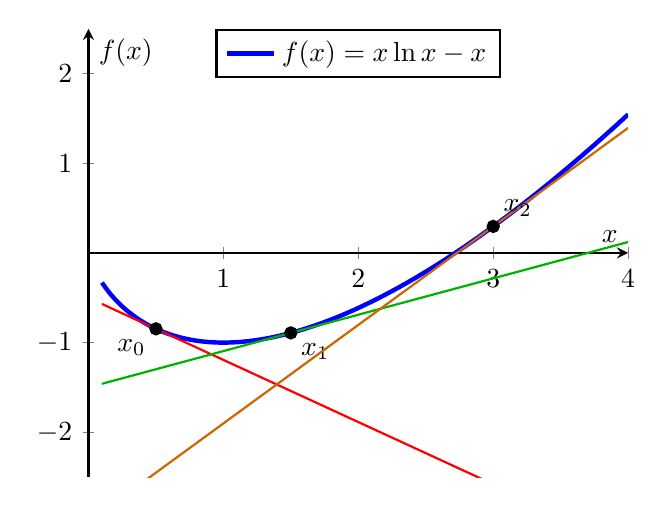
\begin{tikzpicture}
  \begin{axis}[
      axis lines=middle,
      xlabel={$x$},
      ylabel={$f(x)$},
      domain=0.1:4,
      samples=200,
      ymin=-2.5, ymax=2.5,
      xmin=0, xmax=4,
      legend style={at={(0.5,1.0)}, anchor=north},
      thick
    ]
    
    % Function
    \addplot[blue, ultra thick, domain=0.1:4] {x*ln(x) - x};
    \addlegendentry{$f(x) = x \ln x - x$}
    
    % Tangents at x0, x1, x2
    % x0 = 0.5
    \pgfmathsetmacro\xA{0.5}
    \pgfmathsetmacro\yA{\xA*ln(\xA) - \xA}
    \pgfmathsetmacro\mA{ln(\xA)}
    \addplot[red,  thick, domain=0.1:4] {\mA*(x - \xA) + \yA};
    \addplot[only marks, mark=*] coordinates {(\xA,\yA)};
    \node[below left] at (axis cs:\xA,\yA) {$x_0$};

    % x1 = 1.5
    \pgfmathsetmacro\xB{1.5}
    \pgfmathsetmacro\yB{\xB*ln(\xB) - \xB}
    \pgfmathsetmacro\mB{ln(\xB)}
    \addplot[green!70!black,  thick, domain=0.1:4] {\mB*(x - \xB) + \yB};
    \addplot[only marks, mark=*] coordinates {(\xB,\yB)};
    \node[below right] at (axis cs:\xB,\yB) {$x_1$};

    % x2 = 3.0
    \pgfmathsetmacro\xC{3.0}
    \pgfmathsetmacro\yC{\xC*ln(\xC) - \xC}
    \pgfmathsetmacro\mC{ln(\xC)}
    \addplot[orange!80!black,  thick, domain=0.1:4] {\mC*(x - \xC) + \yC};
    \addplot[only marks, mark=*] coordinates {(\xC,\yC)};
    \node[above right] at (axis cs:\xC,\yC) {$x_2$};

  \end{axis}
\end{tikzpicture}\vspace{2ex}
\begin{beamercolorbox}[rounded=true, shadow=true, wd=\textwidth]{block title}\centering
$f^*$ encodes all the information of the convex hull of $f(x)$'s epigraph in terms of its supporting hyperplanes.
\end{beamercolorbox}
\end{frame}

\begin{frame}\frametitle{An Example}
\begin{example}
Let $f(x) = \exp x$. Then $f: \mathbb R \to \mathbb R$ and $f^* : \mathbb R \to \overline{\mathbb R}$ is given by
\[
f^*(x^*) := \sup_{x \in \mathbb R}\{ x^* x - \exp(x) \} = - \inf_{x \in \mathbb R}\{\exp(x) - x^* x\}.
\]
\visible<2->{If $x^* < 0$, then $x\to -\infty$ implies $x^* x - \exp(x) \to +\infty$. Hence, $f^*(x^*) = +\infty$. \medskip}

\visible<3->{If $x^* = 0$, then the least upper bound of $-\exp(x)$ over $x \in \mathbb R$ is 0. Hence, $f^*(x^*) = 0$.  \medskip}

\visible<4->{If $x^* > 0$, then the minimizer of $\exp(x) - x^*x$ solves $\exp(x) = x^*$, i.e., $x = \ln(x^*)$. \medskip}

\visible<5->{So the \alert{convex conjugate} of \alert{$f(x) = \exp(x)$} is Shannon's entropy extended to $\mathbb R$.}
\end{example}
\end{frame}

\begin{frame}\frametitle{The Hellinger Entropy}
\begin{example}
Let $f(x) = -\sqrt{1 - \|x\|^2}$ with $f(x) = +\infty$ for $\|x\| > 1$. Here, we have for $\|x\| \le 1$
\[ 
(\langle x^*, \cdot\rangle - f(\cdot))'(x) = x^* -  (1 - \|x\|^2)^{-1/2} x \Rightarrow x(x^*) = \frac{x^*}{\sqrt{1 + \|x^*\|^2}}
\]
By substitution, we get
\[
f^*(x^*) = \frac{1 + \|x^*\|^2}{\sqrt{1 + \|x^*\|^2}}.
\]
Note: 
\[
\nabla f^*(x^*) = \frac{x^*}{\sqrt{1 + \|x^*\|^2}} \text{ and } \| \nabla f^*(x^*) \| \le 1.
\]
\end{example}
\end{frame}

\begin{frame}\frametitle{Observation}
\begin{beamercolorbox}[rounded=true, shadow=true, wd=\textwidth]{block body}
Given $R_1(a) := a \ln a - a$ and $R_2(a) := -\sqrt{1 - \|a\|^2}$ we see that 
\[
R_1^*(a^*) = \exp(a^*) \text{ and } R_2(a^*) = \frac{1 + \|a^*\|^2}{\sqrt{1 + \|a^*\|^2}}.
\]\visible<2->{
Moreover, though $R_1$, $R_2$ have restricted domains, $R^*_1$, $R^*_2$ are defined on all of $\mathbb R^n$.\medskip}

\visible<3->{What's more: $\nabla R^*_1(a^*) = \exp(a^*)$ and $\nabla R^*_2(a^*) =  \frac{a^*}{\sqrt{1 + \|a^*\|^2}}$}\visible<3->{ and 
\[
\nabla R^*_1(\mathbb R) \subset \mathrm{int \, dom\,} R_1 \text{ and } \nabla R^*_2(\mathbb R^n) \subset \mathrm{int \, dom\,} R_2.
\]}\vspace{-2ex}
\end{beamercolorbox}

\visible<4->{
\begin{beamercolorbox}[rounded=true, shadow=true, wd=\textwidth]{block body}\centering
Is there are general class of functions $R$ for which $\nabla R^*$ maps into  $\mathrm{int \, dom\,} R$? \alert{Yes!}.
\end{beamercolorbox}}
\end{frame}

\begin{frame}\frametitle{Legendre Functions\footnote{\tiny Originally introduced by Rockafellar in 1967, we follow the definition and nomenclature of Teboulle (2018)}}

\visible<1->{
\begin{beamercolorbox}[rounded=true, shadow=true, wd=\textwidth]{block body}\centering
The geometry of a closed convex set $C \subset \mathbb{R}^m$ with a non-empty interior, $\operatorname{int}C \neq \emptyset$, can be encoded into a \alert{Legendre function} $R: \mathbb{R}^m \to \mathbb{R}\cup\{+\infty\}$.
\end{beamercolorbox}}

\begin{minipage}{0.7\textwidth}
\begin{definition}[]
%\label{def:LegendreFunction}
\visible<2->{
Let the essential domain of a function $R$ be defined as $\operatorname{dom} R := \{ a \in \mathbb{R}^m \mid R(a) < \infty \}$.
}\visible<3->{We call a proper convex function a \alert{Legendre function} $R: \mathbb{R}^m \to \mathbb{R}\cup\{+\infty\}$ if}
\begin{itemize}
%% \itemsep=-3pt
\item \visible<4->{$\operatorname{int}(\operatorname{dom} R) \neq \varnothing$;}
\item \visible<5->{$R$ is differentiable on $\operatorname{int}(\operatorname{dom} R)$;}
\item \visible<6->{$\lim_{t \to 0^+} \langle \nabla R(a+t(b-a)), b-a\rangle = -\infty$ for all $a \in \partial( \operatorname{dom} R)$ and $b \in \operatorname{int}(\operatorname{dom} R)$;}
\item \visible<7->{R is strictly convex on $\operatorname{int}(\operatorname{dom} R)$.}
\end{itemize}
\end{definition}
\end{minipage}\hfill
\begin{minipage}{0.3\linewidth}
 \centering
 \begin{figure}
  \centering\vspace{1ex}
  \begin{minipage}[b]{0.6\textwidth}
    \includegraphics[width=\linewidth]{figures/rtr.jpg}
    \captionof*{figure}{\tiny R. Tyrrell Rockafellar}
  \end{minipage}%
  \end{figure}
  \end{minipage}



%Introduced by Rockafellar in 1967~\cite{Rockafellar1967Conjugates}, see also \cite[Chap.~26]{RTRockafellar_1970}, Legendre functions constitute a special class of proper convex functions whose gradients $\nabla R$ become singular on the boundary of their essential domains.
%We denote by $R^*(a^\ast) \coloneqq \sup \{ a \cdot a^\ast - R(a) \mid a \in \mathbb{R}^m \}$ the convex conjugate of $R$.
%
%\begin{theorem}[Rockafellar \text{\cite[Thm. 1]{Rockafellar1967Conjugates}}]
%\label{thm:Rockafellar}
%A proper convex function $R$ is a Legendre function if and only if its convex conjugate $R^\ast$ is also a Legendre function.
%Moreover, $\nabla R \colon \operatorname{int}(\operatorname{dom} R) \to \operatorname{int}(\operatorname{dom} R^*)$ is a topological isomorphism with $(\nabla R)^{-1} = \nabla R^\ast$.
%\end{theorem}
%
%
%From now on, we assume that ${R(a)}/{|a|} \to +\infty$ as $|a| \to \infty$ and $\operatorname{dom} R = C$.
\end{frame}

\begin{frame}\frametitle{Properties of Legendre Functions}

\visible<1->{
\begin{beamercolorbox}[rounded=true, shadow=true, wd=\textwidth]{block body}\centering
 Legendre functions constitute a special class of proper convex functions whose gradients $\nabla R$ become singular on the boundary of their essential domains.
\end{beamercolorbox}}

\begin{minipage}{0.7\textwidth}
\begin{theorem}[Rockafellar (1967)]
\label{thm:Rockafellar}
A proper convex function $R$ is a Legendre function if and only if its convex conjugate $R^\ast$ is also a Legendre function.
Moreover, $\nabla R \colon \operatorname{int}(\operatorname{dom} R) \to \operatorname{int}(\operatorname{dom} R^*)$ is a topological isomorphism with $(\nabla R)^{-1} = \nabla R^\ast$.
\end{theorem}
\end{minipage}\hfill
\begin{minipage}{0.3\linewidth}
 \centering
 \begin{figure}
  \centering\vspace{1ex}
  \begin{minipage}[b]{0.6\textwidth}
    \includegraphics[width=\linewidth]{figures/rtr.jpg}
    \captionof*{figure}{\tiny R. Tyrrell Rockafellar}
  \end{minipage}%
  \end{figure}
  \end{minipage}

\visible<2->{
\begin{beamercolorbox}[rounded=true, shadow=true, wd=\textwidth]{block title}\centering
It can also be shown that ${R(a)}/{|a|} \to +\infty$ as $|a| \to \infty$ if and only if $\operatorname{dom} R^* = \mathbb R^n$.
\end{beamercolorbox}}

\end{frame}

\begin{frame}\frametitle{Geometry Preserving Transformations}

\begin{beamercolorbox}[rounded=true, shadow=true, wd=\textwidth]{block title}
\begin{equation*} \label{eq:intro:feasible_set}
K = \{ v \in V \mid Bv(x) \in C(x) \text{ for almost every } x \in \Omega_d \subset \overline{\Omega} \}.
\end{equation*}
\end{beamercolorbox}\hfill

\begin{minipage}{0.5\linewidth}
\begin{beamercolorbox}[rounded=true, shadow=true, wd=\textwidth]{block title}
\centering
 $\nabla R \colon \operatorname{int}C \to \operatorname{int}(\operatorname{dom} R^*)$ satisfies %is a topological isomorphism 
 $(\nabla R)^{-1} = \nabla R^\ast$
\end{beamercolorbox}
\end{minipage}
%
\begin{minipage}{0.4\linewidth}
\begin{figure}[h]
\includegraphics[width=0.8\linewidth]{figures/Geodesic3.png} 
\end{figure}
\end{minipage}
\end{frame}

\section{The General LVPP Algorithm}

\begin{frame}[plain,c]
%\frametitle{A first slide}
\hfill
\begin{center}
\Large With the help of Legendre functions, we can find mappings that \alert{guarantee} feasibility for pointwise inequality constraints.
\end{center}
\hfill
\end{frame}

\begin{frame}\frametitle{}
\thispagestyle{empty}
%\hypertarget{lvpp-table}{}
%\hyperlink{lvpp-examples}{\beamerbutton{Go to Examples}}
\begin{table}
\centering
\small
% \renewcommand{\arraystretch}{0.6}
\setlength{\tabcolsep}{5pt}
\renewcommand{\arraystretch}{1.4}
    \begin{tabular}{ c|c|c|c } 
     \toprule
      Feasible set $K$ & Legendre function $R$ & $B$ & $\nabla R^*(\psi)$ \\ 
     \midrule
     $\big\{ u \geq \phi \big\}$ & $(a - \phi) \ln (a - \phi) - (a - \phi)$ & $\operatorname{id}$ & $\phi + \exp\psi$ \\[2ex]
     $\big\{ \phi_1 \leq u \leq \phi_2 \big\}$ & $(a - \phi_1) \ln (a - \phi_1) + (\phi_2-a) \ln (\phi_2-a)$ & $\operatorname{id}$ & $\dfrac{\phi_1 + \phi_2\exp\psi}{1 + \exp\psi}$ \\[2ex]
     % $\big\{ \phi_1 \leq u \leq \phi_2 \big\}$ & $\sum_{i=1}^2 (-1)^i (\phi_i - a) \ln \left( (-1)^i (\phi_i - a)\right)$ & $\operatorname{id}$ & $\dfrac{\phi_1 + \phi_2\exp\psi}{1 + \exp\psi}$ \\[2ex]
     $\big\{\gamma u \ge \phi \big\}$ & $(a-\phi) \ln (a - \phi) - (a - \phi)$ & $\gamma$ &  $\phi + \exp\psi$ \\[2ex]
     $\big\{ (\gamma u)\cdot n \leq \phi \big\}$ & $(\phi-a) \ln (\phi - a) - (\phi - a)$ & $\gamma(\cdot) \cdot n$ & $\phi - \exp(-\psi)$ \\[2ex]
     $\big\{| \nabla u | \le \phi \big\}$ & $ -\sqrt{\phi^2 - | a |^2}$ & $\nabla$  & $\dfrac{\phi\psi}{\sqrt{1 + | \psi |^2}}$ \\[3ex] 
     $\big\{ u \ge 0,\; \sum_{i} u_i = 1 \big\}$ & $\sum_{i} a_i \ln(a_i)$ & $\operatorname{id}$ & $\dfrac{\exp\psi}{\sum_{i} \exp\psi_i}$\\[2ex]
     $\big\{ \det (\nabla^2 u) \geq 0 \big\}$ & $\operatorname{tr}(a\ln a - a)$ & $\nabla^2$ & $\exp \psi$ \\[2ex]
     \bottomrule
    \end{tabular}
\vspace{-1em}
%\end{sidewaystable}
\end{table}
\end{frame}

\begin{frame}\frametitle{The LVPP Algorithm}
\begin{beamercolorbox}[rounded=true, shadow=true, wd=\textwidth]{block body}
Taking $\mathop{\text{dom}}R(\cdot,x) := C(x)$ brings us back to proximal point:\medskip

\visible<2->{Given $u^0 \in V$ and $\left\{\alpha_k\right\}$ find $u \in \mathop{\text{argmin}}_{v \in K} J(v)$  by recursively computing} 
\visible<3->{
\begin{equation}\label{eq:lvpp-op}
\only<3>{
u^{k} \in \mathop{\text{argmin}}_{u \in K} J(u) + \alpha_{k}^{-1} \int_{\Omega_d} D_R(Bu, Bu^{k-1}) \dd \mathcal{H}_d, \quad k = 1, 2, \dots.
}
\only<4->{
    \text{Find } u^k \in K: \quad \underbrace{\alpha_k J^\prime(u^k) +  B^* \nabla R(Bu^k) - B^* \nabla R(Bu^{k-1}) = 0,}_{\text{Properties of $R$ force constraints to be inactive for $u^k$} }
}
\end{equation}\vspace{-2ex}
}\end{beamercolorbox}
\visible<5->{
\begin{beamercolorbox}[rounded=true, shadow=true, wd=\textwidth]{block body}
Using again \alert{latent variables}: given $\psi^0 \in W$, find $(u^{k}, \psi^{k}) \in V \times W$ satisfying
\begin{subequations} \label{eq:intro:lvpp}
\begin{align}
\label{eq:intro:lvpp:a}
\alpha_{k} J'(u^{k}) + B^*\psi^{k} &= B^*\psi^{k-1}, \\
\label{eq:intro:lvpp:b}
Bu^{k} - \nabla R^*(\psi^{k}) &= 0
\end{align}
\end{subequations}\vspace{-4ex}
\end{beamercolorbox}\centering
}\visible<6->{
\begin{minipage}{0.4\linewidth} 
\begin{beamercolorbox}[rounded=true, shadow=true, wd=\textwidth]{block title}
\centering
\textbf{\eqref{eq:intro:lvpp:b} implies }$Bu^k \in  \nabla R^*(W) \subset C$!\\
Clearly, $\nabla R^*(W_h) \subset C$, as well.
\end{beamercolorbox}
\end{minipage}
}
\visible<7->{ 
\begin{minipage}{0.5\linewidth} 
\begin{beamercolorbox}[rounded=true, shadow=true, wd=\textwidth]{block title}
\centering
A new, unifying perspective on pointwise inequality constraints.
\end{beamercolorbox}
\end{minipage}
}
\end{frame}

%\begin{frame}\frametitle{A}
%\begin{itemize}
%\item Define proper, convex, lsc again
%\item Define convex conjugate and motivate its meaning
%\item Define Legendre function
%\item Find a picture of Rockafellar
%\item Work out two examples to show how to compute the convex conjugate
%\item Prove (if possible) the crucial Rockafellar theorems
%\item Give the table in the paper
%\item Return to Bregman 
%\end{itemize}
%\end{frame}





\section{Applications}

\begin{frame}\frametitle{The Signorini Problem}
\begin{minipage}{0.55\linewidth}
\visible<1->{
\begin{beamercolorbox}[rounded=true, shadow=true, wd=\textwidth]{block body}
Signorini (1959), analyzed by Fichera (1963).\\
 
The essential first problem in contact mechanics.\\
 
Models the deformation of a linear elastic body in the presence of a contact boundary constraint.
\end{beamercolorbox}
}\visible<2->{
\begin{beamercolorbox}[rounded=true, shadow=true, wd=\textwidth]{block body}
\visible<2->{$\Omega \subset \mathbb{R}^3$, $\Gamma$ split into two disjoint subsets.}
\visible<2->{$\Gamma = \overline{ \Gamma_\mathrm{D} \cup \Gamma_\mathrm{T} }$ with\\
$\Gamma_D$ for \textbf{d}isplacement\\
$\Gamma_{T}$ for \textbf{t}raction boundary conditions.}
\end{beamercolorbox}}
\end{minipage}\hspace{4ex}
\begin{minipage}{0.3\linewidth}
 \centering
 \begin{figure}
  \centering\vspace{1ex}
  \visible<1->{\begin{minipage}[b]{0.45\textwidth}
    \includegraphics[width=\linewidth]{figures/Antonio_Signorini.jpg}
    \captionof*{figure}{\tiny A. Signorini}
  \end{minipage}}%
  \hfill
  \begin{minipage}[b]{0.46\textwidth}
    \includegraphics[width=\linewidth]{figures/Gaetano_Fichera.jpg}
    \captionof*{figure}{\tiny G. Fichera}
  \end{minipage}
\end{figure}\vspace{-8ex}
\begin{figure}
	\centering
	\begin{tikzpicture}
		\node at (-3.35,0) {\includegraphics[height=1.25in]{figures/contact.png}};
    \end{tikzpicture}
\end{figure}
\end{minipage}
\end{frame}

\begin{frame}\frametitle{The Signorini Problem}
\begin{minipage}{0.55\linewidth}
\visible<1->{
\begin{beamercolorbox}[rounded=true, shadow=true, wd=\textwidth]{block body}
\visible<1->{State space:\vspace{-1.5ex}
\begin{equation*}
\label{eq:Signorini_V}
    V = \big\{ u \in H^1(\Omega,\mathbb{R}^3)
        \mid u = g \text{ on } \Gamma_\mathrm{D\textbf{}}
    \big\}
    \,,
\end{equation*}}\vspace{-4ex}

\visible<2->{Objective function:\vspace{-1.5ex}
\begin{equation*}
    J(u) =
    \frac{1}{2}\int_\Omega (\mathbb C \epsilon(u)) : \epsilon(u) \dd x
    -
    \int_\Omega f \cdot u \dd x
    \,,
\end{equation*}}\vspace{-2.5ex}

\visible<3->{Inequality constraints:\vspace{-1ex}
\begin{equation*}
 \alert{   K = \big\{ u \in V
        \mid u \cdot \tilde{n} \leq \phi_1 \text{ on } \Gamma_\mathrm{T}
    \big\} }
    \,.
\end{equation*}}\vspace{-4ex}
\end{beamercolorbox}
}\visible<4->{
\begin{beamercolorbox}[rounded=true, shadow=true, wd=\textwidth]{block body}\scriptsize
%Here, $\epsilon : H^1(\Omega,\mathbb{R}^3) \to L^2(\Omega,\mathbb{R}^{3\times 3}_{\mathrm{sym}})$, 
$\epsilon := (\nabla + \nabla^\top)/2$ symmetric gradient\smallskip
 
$\C \colon \mathbb{R}^{3\times 3}_{\mathrm{sym}} \to \mathbb{R}^{3\times3}_{\mathrm{sym}}$ sym.\ pos.-def.\ elasticity tensor\smallskip

$f \colon \Omega \to \mathbb{R}^3$ internal body force density\smallskip

$\phi_1 \colon \Gamma_\mathrm{T} \to \mathbb{R}_+$ gap function, $\tilde{n}$ normal to contact surface.
\end{beamercolorbox}}
\end{minipage}\hspace{4ex}
\begin{minipage}{0.3\linewidth}
 \centering
 \begin{figure}
  \centering\vspace{1ex}
  \visible<1->{\begin{minipage}[b]{0.45\textwidth}
    \includegraphics[width=\linewidth]{figures/Antonio_Signorini.jpg}
    \captionof*{figure}{\tiny A. Signorini}
  \end{minipage}}%
  \hfill
  \begin{minipage}[b]{0.46\textwidth}
    \includegraphics[width=\linewidth]{figures/Gaetano_Fichera.jpg}
    \captionof*{figure}{\tiny G. Fichera}
  \end{minipage}
\end{figure}\vspace{-8ex}
\begin{figure}
	\centering
	\begin{tikzpicture}
		\node at (-3.35,0) {\includegraphics[height=1.25in]{figures/contact.png}};
    \end{tikzpicture}
\end{figure}
\end{minipage}
\end{frame}

\begin{frame}\frametitle{LVPP for Signorini}
\begin{minipage}{\linewidth}
\begin{beamercolorbox}[rounded=true, shadow=true, wd=\textwidth]{block body}

\begin{columns}
\begin{column}{0.55\textwidth}
\begin{itemize}
\item $B := \gamma(\cdot) \cdot \tilde{n}$ (trace on contact boundary)
\item $\Omega_d := \Gamma_\mathrm{T}$
\item $C(x) := (-\infty,\phi_1(x)]$
\item $R(a) := (a-\phi) \ln (a - \phi) - (a - \phi)$
\item $\psi^0 = 0$
\end{itemize}
\end{column}
\begin{column}{0.3\textwidth}  %%<--- here
\begin{minipage}{0.3\linewidth}
 \centering
\begin{figure}
	\centering
	\begin{tikzpicture}
		\node at (-7.35,0) {\includegraphics[height=1.25in]{figures/contact.png}};
    \end{tikzpicture}
\end{figure}
\end{minipage}
\end{column}
\end{columns}
%The LVPP saddle-point problems:\\
Find $(u^{k}, \psi^{k}) \in V \times L^\infty(\Gamma_\mathrm{T})$ satisfying
\begin{subequations}
\label{eq:SignoriniVF}
\begin{align}
    ( \alpha_k\C \epsilon(u^k), \epsilon(v) ) - (\psi^k, v\cdot \tilde{n} )_{\Gamma_\mathrm{T}}
    &=
    (\alpha_k f, v) - ( \psi^{k-1}, v \cdot \tilde{n} )_{\Gamma_\mathrm{T}}
    \,,
    \\
    ( u^k\cdot \tilde{n} , w )_{\Gamma_\mathrm{T}} + ( \exp \psi^k, w )_{\Gamma_\mathrm{T}}
    &= ( \phi_1, w )_{\Gamma_\mathrm{T}}
    \,,
\end{align}
\end{subequations}
for all $(v, w) \in V \times L^\infty(\Gamma_\mathrm{T})$, where $(\cdot, \cdot  )_{\Gamma_\mathrm{T}}$ denotes the $L^2(\Gamma_\mathrm{T})$-inner product.
\end{beamercolorbox}
\end{minipage}
\end{frame}

\begin{frame}\frametitle{LVPP for Signorini}
\begin{beamercolorbox}[rounded=true, shadow=true, wd=\textwidth]{block body}
\begin{itemize}
%\item Code available here: 
\item Define a \alert{proximal Galerkin method} using equal-order continuous Lagrange spaces for the displacement $u$ and latent variable $\psi$.
\item \visible<2->{Note that the spaces are on manifolds of differing dimensions. Hence, the two discrete subspaces are not the same.}
\item \visible<3->{We used the mixed-dimensional assembly routines in DOLFINx.}
%\item \visible<4->{The discrete problem is solved for half of a sphere centered at $(0,0,0.5)$ with radius $0.4$ coming into contact with the rigid $x,y$-plane.} 
%\item \visible<5->{$\tilde{n}=(0,0,-1)^\top$ and $\phi_1$ measures the vertical distance between the $x,y$-plane and the boundary of the half sphere, i.e., $\phi_1(x,y,z) = z$.}
%\item \visible<6->{Second-order Lagrange elements approximate the geometry, the displacement, and the latent variable.}
%\item The initial proximity parameter $\alpha_0 = 0.005$ is doubled at each subsequent proximal step (i.e., LVPP iteration). 
%\item  The tolerance for Newton’s method is set to $10^{-6}$. 
%\item  The LVPP algorithm requires a total of 13 proximal iterations, amounting to 17 linear solves. The maximum number of Newton steps was 5, the minimum 1. The number of degrees of freedom was $17,613$ for a mesh with $3,661$ cells.
\end{itemize}
\end{beamercolorbox}
\end{frame}

\begin{frame}\frametitle{LVPP for Signorini}
\begin{minipage}{0.55\linewidth}
\begin{beamercolorbox}[rounded=true, shadow=true, wd=\textwidth]{block body}
 \visible<1->{Initial shape: hemisphere centered at $(0,0,0.5)$ with radius $0.4$ coming in contact with $xy$-plane.} \smallskip
 
 \visible<1->{$\tilde{n}=(0,0,-1)^\top$ and $\phi_1(x,y,z) = z$.}\smallskip
 
\visible<1->{Second-order Lagrange elements for geometry, displacement, and the latent variable.}
\end{beamercolorbox}
\visible<2->{
\begin{beamercolorbox}[rounded=true, shadow=true, wd=\textwidth]{block title}
Performance of LVPP:\\
Proximal iterations 13 ($\alpha$ updates)\\
\textbf{Total linear solves: 17}\\
Max Newton steps: 5\\
Min Newton steps: 1
DoFs: 17,613\\
Cells: 3,661
\end{beamercolorbox}}
\end{minipage}\hspace{4ex}
\begin{minipage}{0.3\linewidth}
 \centering
\begin{beamercolorbox}[rounded=true, shadow=true, wd=\textwidth]{block body}
Parameters:\\
$\alpha_0 = 5$E-3\\
$\alpha_{k+1} := 2\alpha_k$\\
${\tt tol_{rel}} = {\tt tol_{abs}}$ = 1E-6
\end{beamercolorbox}
\begin{figure}
	\centering
	\begin{tikzpicture}
		\node at (-3.35,0) {\includegraphics[height=1.25in]{figures/contact.png}};
    \end{tikzpicture}
\end{figure}
\end{minipage}
\end{frame}

\begin{frame}{Variational Fracture}

  \begin{minipage}{0.53\textwidth}
  \begin{beamercolorbox}[rounded=true, shadow=true, wd=\textwidth]{block title}\scriptsize
A.\ A.\ Griffith's foundational paper (1921) uses a preexisting crack and well-defined crack path.\medskip

Mostly overcome in the seminal work by Francfort and Marigo (1998)\medskip

The widely used \textbf{phase-field approximation} by Bourdin, Francfort, and Marigo (2000).
%\footnote{\tiny The model in Bourdin, Francfort, and Marigo (2000) is an Ambrosio-Tortorelli approximation of the Mumford-Shah functional \cite{Mumford1989,Ambrosio1990}.}

%We only solve for the vertical displacements here. 
     \end{beamercolorbox}
 
 \visible<2->{    
\begin{beamercolorbox}[rounded=true, shadow=true, wd=\textwidth]{block body}\scriptsize
\visible<2->{Challenge 1: Variational fracture is a \alert{free discontinuity problem (FDP)}. The state is split into a \alert{function} $u$ over $\Omega$ and a \alert{geometric quantity} $\Gamma \subset \Omega$.\medskip}
 
 \visible<3->{Challenge 2: The phase-field approximation has a \alert{non-convex energy} and admits \alert{non-unique global solutions}. \medskip}
 
 \visible<4->{Challenge 3: The \alert{irreversibility} of the crack evolution has to be built into the pointwise inequality constraints.}
      \end{beamercolorbox}}
    \end{minipage}\hspace*{1.75cm}
    \begin{minipage}{0.3\textwidth}
  \centering
 \begin{figure}
  \centering\vspace{1ex}
   \begin{minipage}[b]{0.4\textwidth}
    \includegraphics[width=\linewidth]{figures/griffith.jpg}
    \captionof*{figure}{\tiny A.A.\ Griffith}
  \end{minipage}
  \hfill
  \begin{minipage}[b]{0.4\textwidth}
    \includegraphics[width=\linewidth]{figures/francfort.jpg}
    \captionof*{figure}{\tiny G.\ Francfort }
  \end{minipage}
  \vspace{1em}
  \begin{minipage}[b]{0.4\textwidth}
    \includegraphics[width=\linewidth]{figures/marigo.jpeg}
    \captionof*{figure}{\tiny J.-J.\ Marigo}
  \end{minipage}
  \hfill
  \begin{minipage}[b]{0.4\textwidth}
    \includegraphics[width=\linewidth]{figures/BlaiseBourdin_1024.jpg}
    \captionof*{figure}{\tiny B.\ Bourdin }
  \end{minipage}
\end{figure}
    \end{minipage}
\end{frame}

\begin{frame}\frametitle{Problem Description}
\begin{minipage}{0.6\textwidth}
\begin{beamercolorbox}[rounded=true, shadow=true, wd=\textwidth]{block body}\scriptsize
Domain: $\Omega \subset \mathbb R^n$ open, bounded set\medskip 

\visible<2->{(Francfort \& Marigo): $u : \Omega \to \mathbb R$ (displacement), $\Gamma \subset \Omega \cap \mathbb R^{n-1}$ (crack). Note \alert{this is not a function!}\medskip}

\visible<3->{(Bourdin, Francfort \& Marigo): The \alert{geometric variable} $\Gamma$ is replaced by an \alert{order parameter} $c : \Omega \to [0,1]$ 
\[
c = 0 \text{ no damage, } \alert{c = 1} \text{ presence of crack.}
\] 
The localization of the crack controlled by a \alert{length scale} $\ell > 0$ \medskip}

\visible<4->{The crack evolution is computed over a \alert{quasi-static incremental loading} procedure.\medskip}

\visible<5->{At each step, the load on the body is varied, and the body is allowed to equilibrate.\medskip}
\end{beamercolorbox}
\end{minipage}\hspace{4ex}
\begin{minipage}{0.27\textwidth}
\begin{figure}
  \includegraphics[width=\linewidth]{figures/christian-lambert-KtqTxJgN70M-unsplash.jpg}
  \captionof*{figure}{\tiny Photo by Christian Lambert}
  \end{figure}
\end{minipage}

%%Photo by <a href="https://unsplash.com/@_christianlambert?utm_content=creditCopyText&utm_medium=referral&utm_source=unsplash">Christian Lambert</a> on <a href="https://unsplash.com/photos/blue-and-white-abstract-painting-KtqTxJgN70M?utm_content=creditCopyText&utm_medium=referral&utm_source=unsplash">Unsplash</a>
      
\end{frame}

\begin{frame}\frametitle{Problem Description}
\begin{beamercolorbox}[rounded=true, shadow=true, wd=\textwidth]{block body}
At each loading step, we are given Dirichlet boundary data $g$ and the previous order parameter $c_{\rm prev}$. \visible<2->{This defines our feasible set $K$:
\begin{equation*}
\label{eq:FeasibleSetFracture}
K = \left\{ (u,c) \in H^1_g(\Omega) \times H^1(\Omega) \mid 0 \le c_{\rm prev} \le c \le 1 \; \text{a.e.~in} \; \Omega \right\},
\end{equation*}
where
%\begin{equation*}
$V = H^1_g(\Omega) = \left\{ u \in H^1(\Omega) \mid \gamma u = g \text{ on } \Gamma_D \right\},$
%\end{equation*}
with $\Gamma_D \subset \partial \Omega$.}
\end{beamercolorbox}

\visible<3->{
\begin{beamercolorbox}[rounded=true, shadow=true, wd=\textwidth]{block body}
Given energy release rates $G_c > 0$, 
%the length scale $\ell > 0$,  
%an artificial residual stiffness
artificial  stiffness
%of a fully ruptured phase 
$\epsilon > 0$, we arrive at the (\alert{non-convex}) objective functional:
\[
J(u,c) := \underbrace{\frac{1}{2}\int_{\Omega}(\epsilon + (1-\epsilon)
(1-c)^2)|\nabla u|^2\,\mathrm{d}x}_{\text{biconvex bulk energy}} 
+ 
\underbrace{\frac{G_c}{2}\int_{\Omega} \ell |\nabla c|^2 
+ 
\ell^{-1}|c|^2\,\mathrm{d}x.}_{\text{governs diffuse crack interface}}
\]\vspace{-2ex}
\end{beamercolorbox}}
\end{frame}

\begin{frame}\frametitle{LVPP for Variational Fracture}
\vspace{-1ex}
\begin{minipage}{0.25\textwidth}\scriptsize
\begin{beamercolorbox}[rounded=true, shadow=true, wd=\textwidth]{block title}
%\begin{itemize}
%\item 
$B := (0,\operatorname{id})$ (acts only on $c$)\medskip

%\item 
$\Omega_d :=\Omega$\medskip

%\item 
$C(x) := \mathbb R \times [c_{\rm prev}(x),1]$\medskip

%\item 
$R(a) := (a - \phi_1) \ln (a - \phi_1) + (\phi_2-a) \ln (\phi_2-a)$\medskip

%\item 
$\phi_1 := c_{\rm prev}$ and $\phi_2 := 1$\medskip

%\item 
No latent variable for $u$\medskip

%\item 
$\psi^0 = 0$
%\end{itemize}
\end{beamercolorbox}
\end{minipage}\hfill\visible<2->{
\begin{minipage}{0.72\textwidth}  %%<--- here
\begin{beamercolorbox}[rounded=true, shadow=true, wd=\textwidth]{block body}\scriptsize\visible<3->{
Find $(u^k, c^k, \psi^k) \in H^1_g(\Omega) \times H^1(\Omega) \times L^\infty(\Omega)$ such that}
\begin{subequations}
\label{eq:FractureVF}
\begin{align*}
    \visible<4->{&\underbrace{\alpha_k G ((\epsilon + (1-\epsilon)(1-c^k)^2)\nabla u^k, \nabla v)}_{= \alpha_k(\partial_u J(u,c),v)}
    = 0
    \,,}
    \\\visible<5->{
    &
    %\begin{split}
    \underbrace{-\alpha_k  ((1-\epsilon)(1-c^k)|\nabla u^k|^2,d)%\hspace{30mm}
%    \indent 
    +
    \alpha_k G_c ( \ell(\nabla c^k, \nabla d) + \ell^{-1}(c^k, d) )}_{=\alpha_k (\partial_c J(u,c),d)}}
    +\\\visible<5->{
    &\hspace{7cm}(\psi^k-\psi^{k-1},d)%\\
    =
    0
    \,,}
    %\end{split}
    \\\visible<6->{
    &\underbrace{(c^k,w)
    -
    \bigg(\frac{c_\mathrm{prev} + \exp (\psi^k)}{\exp(\psi^k) + 1}, w\bigg)}_{= (c - \nabla R^*(\psi),w)}
    =
    0
    \,,}
\end{align*}
\end{subequations}\visible<7->{
for all $(v, d, w) \in H^1_0(\Omega) \times H^1(\Omega) \times L^\infty(\Omega)$.}
\end{beamercolorbox}
\end{minipage}}

\visible<8->{
\begin{beamercolorbox}[rounded=true, shadow=true, wd=\textwidth]{block title}\centering
Many choose an alternating minimization scheme (leaving off the 3$^{rd}$ equation) due to the simplicity of the individual equations. We use Newton.
\end{beamercolorbox}}
\end{frame}

\begin{frame}\frametitle{LVPP for Variational Fracture}

\begin{beamercolorbox}[rounded=true, shadow=true, wd=\textwidth]{block body}
\begin{itemize}
%\item Code available here: 
\item Define a \alert{proximal Galerkin method} continuous piecewise linear finite elements for $u$, $c$, and $\psi$.
%\item \visible<2->{Solve the resulting discrete systems with Newton's method.}
\item \visible<3->{For robustness of the optimization procedure, we perturb the  system Jacobian with a coercive modification, by adding
\[
\iota ((u, v) + (c, d) - (\psi, w))
\]
to the Jacobian with perturbation parameter $\iota = 10^{-3}$.}
\item \visible<4->{Simple heuristic for $\alpha_k$:  if the number of Newton iterations is four or fewer, $\alpha_{k+1} = 2\alpha_k$; if the number of Newton iterations is ten or more, $\alpha_{k+1} = \alpha_k/2$; otherwise $\alpha_{k+1} = \alpha_k$.
}
\end{itemize}
\end{beamercolorbox}
\end{frame}

\begin{frame}\frametitle{LVPP for Variational Fracture}
\begin{minipage}{0.55\linewidth}
\begin{beamercolorbox}[rounded=true, shadow=true, wd=\textwidth]{block body}
 \visible<1->{The anti-plane shear test: impose $u = +L$ top right of notch, $u = -L$ top left of notch} \smallskip
 
 \visible<1->{At each loading step, $L := L + 0.005$, starting from zero.
Natural BCs elsewhere.}

Stop when $L = 2$.
\end{beamercolorbox}
\visible<2->{
\begin{beamercolorbox}[rounded=true, shadow=true, wd=\textwidth]{block title}
Performance of LVPP:\\
Average proximal steps per loading: 2.85\\
Maximum number of proximal steps: 147\\
Average number of Newton steps: 5.44
\end{beamercolorbox}}
\end{minipage}\hspace{4ex}
\begin{minipage}{0.3\linewidth}
 \centering
%\begin{beamercolorbox}[rounded=true, shadow=true, wd=\textwidth]{block body}
%Parameters:\\
%
%\end{beamercolorbox}
\begin{figure}
\centering
\begin{minipage}[c]{3cm}
\begin{tikzpicture}
    \node[anchor=south west,inner sep=0] (image) at (0,0) {\includegraphics[width=\textwidth]{Figures/fracture-damage-4ref.png}};
    \begin{scope}[x={(image.south east)},y={(image.north west)}]
        \node (bcleft) at (0.25, 1.05) {\small $u = -L$};
        \node (bcright) at (0.75, 1.05) {\small $u = +L$};
    \end{scope}
\end{tikzpicture}
\end{minipage}
\hspace*{0cm}
 \begin{minipage}[c]{0.9cm}
     \includegraphics[width=\linewidth]{figures/fracture-damage-colorbar-label.png}
 \end{minipage}
%\caption{The final damage field for the fracture problem described in \Cref{sec:fracture}.}
%\label{fig:fracture}
% \vspace*{-1em}
\end{figure}
\end{minipage}
\end{frame}

\begin{frame}\frametitle{Fully Nonlinear PDEs}
\begin{minipage}{0.5\linewidth}
\begin{beamercolorbox}[rounded=true, shadow=true, wd=\textwidth]{block body}
Many nonlinear  
PDEs have the form:\\ Find $u: \Omega \to \mathbb R$ such that
\begin{equation*}\label{eq:nonlinear-pde}
F(x,u,\nabla u) = 0 \text{ in } \Omega
\text{ and } u = g \text{ on }\partial \Omega\,.
\end{equation*}

This equation lack a divergence structure.\medskip

Integrating by parts will not lead us to the correct notion of a weak solution.%\medskip
%We need the concept of viscosity solution introduced by Crandall and Lions (1983).
\end{beamercolorbox}\hfill\visible<2->{
\begin{beamercolorbox}[rounded=true, shadow=true, wd=\textwidth]{block title}
We need the concept of viscosity solution introduced by Crandall and Lions (1983).
\end{beamercolorbox}}
\end{minipage}\hspace{3ex}
\begin{minipage}{0.35\linewidth}
 \centering
 \begin{figure}
  \centering\vspace{1ex}
  \visible<1->{\begin{minipage}[b]{0.5\textwidth}
    \includegraphics[width=\linewidth]{figures/pllions.jpg}
    \captionof*{figure}{\tiny P.-L. Lions}
  \end{minipage}}%
  \hfill
  \begin{minipage}[b]{0.44\textwidth}
    \includegraphics[width=\linewidth]{figures/mgcrandall.jpg}
    \captionof*{figure}{\tiny M.G.\ Crandall}
  \end{minipage}\vspace{-2ex}
    \includegraphics[width=0.7\linewidth]{figures/eikonal_mobius.png}
\end{figure}
\end{minipage}
\end{frame}

\begin{frame}{Viscosity Solutions}
%\begin{definition}
\visible<1->{\textbf{Subsolution:} An \alert{upper semicontinuous} function $u$ in $\Omega$ is a \alert{viscosity subsolution} if for any $x_0 \in \Omega$ and any $C^2$ function $\phi$ such that $\phi(x_0) = u(x_0)$ and $\phi \geq u$ in a neighborhood of $x_0$, we have:
\[
F\left(x_0, \phi(x_0), D\phi(x_0)\right) \leq 0.
\]}\vspace{-1ex}

%\vspace{0.5em}

\visible<2->{\textbf{Supersolution:} A \alert{lower semicontinuous} function $u$ in $\Omega$ is a \alert{viscosity supersolution} if for any $x_0 \in \Omega$ and any $C^2$ function $\phi$
such that $\phi(x_0) = u(x_0)$ and $\phi \leq u$ in a neighborhood of $x_0$, we have:
\[
F\left(x_0, \phi(x_0), D\phi(x_0))\right) \geq 0.
\]}\vspace{-1ex}

%\vspace{0.5em}

\visible<3->{\textbf{Viscosity Solution:} A \alert{continuous} function $u$ is a \alert{viscosity solution} of the PDE
\[
F(x, u, Du) = 0 \quad \text{in } \Omega
\]
if it is both a subsolution and a supersolution.}
%\end{definition}
\end{frame}


\begin{frame}\frametitle{An Example}
\begin{example}[Eikonal Equation]
Given $\Omega \subset \mathbb R^n$, a continuous function $\rho : \Omega \to \mathbb R$, and boundary data $g \in W^{1,\infty}(\Omega)$ such that $|\nabla g| \le \rho$,  find $u : \Omega \to \mathbb R$ such that
\begin{equation*}\label{eq:eik}
\aligned
|\nabla u| &= \rho \text{ in } \Omega,\\
u &= g \text{ on } \partial \Omega.
\endaligned
\end{equation*}
This equation admits a unique viscosity solution $\bar{u}$.
\end{example}\visible<2->{
\begin{beamercolorbox}[rounded=true, shadow=true, wd=\textwidth]{block title}\centering
But what does this have to do with inequality constraints or variational inequalities?
\end{beamercolorbox}}

\end{frame}

\begin{frame}\frametitle{Gradient Constraints}
% \hypertarget{eikonal}{}  % Target anchor”
    % Button to go back
%    \hyperlink{extensions}{\beamerbutton{Back to Extensions}}
\begin{beamercolorbox}[rounded=true, shadow=true, wd=\textwidth]{block body}
$\Omega \subset \mathbb R^n$ is an open bounded subset.\medskip

$\rho : \Omega \to \mathbb R_+$ is continuous and $\rho \ge \underline{\rho} > 
0$ for constant $\underline{\rho}$ (a.e.\ $\Omega$).\medskip

Define an objective function
\[
J(v) := -\int_{\Omega} v \, \mathrm{d} x 
\] 
over
\[
K = \left\{
v \in W^{1,\infty}_g(\Omega) \left|\; | \nabla v | \le \rho \text{ a.e. } \Omega \right.
\right\}
\] 
where $g \in W^{1,\infty}(\Omega)$ satisfies the bound constraint.\medskip

Then $u$ the \alert{minimizer} of $J$ over $K$ is a \alert{viscosity solution} of the \alert{eikonal equation}.\footnote{\tiny S. Zagatti (2014)}
\end{beamercolorbox}

%S. Zagatti (2014)\footnote{\tiny Theorem 1., \textit{Maximal generalized solution of eikonal equation}  J. Differential Equations 257 (2014) 231–263 } if $\rho$ is continuous on $\Omega$ up to a closed null set $N$, then $u$ is a generalized solution of the \textbf{Eikonal equation}:
\end{frame}

\begin{frame}\frametitle{LVPP for Eikonal Equation}
\vspace{-1ex}
\begin{minipage}{0.25\textwidth}\scriptsize
\begin{beamercolorbox}[rounded=true, shadow=true, wd=\textwidth]{block title}
$V := H^1_0(\Omega)$\medskip

$B := \nabla$\medskip

$C := \mathbb B_{1}(0)$\medskip

$\Omega_d := \Omega$\medskip
 
$R(a) := -\sqrt{1 - \|a\|^2}$\medskip

$\rho := 1$\medskip

$\psi^0 := 0$
\end{beamercolorbox}
\end{minipage}\hfill\visible<2->{
\begin{minipage}{0.72\textwidth}  %%<--- here
\begin{beamercolorbox}[rounded=true, shadow=true, wd=\textwidth]{block body}
Find \only<2,3>{$(u^{k}, \psi^{k}) \in H^1_0(\Omega) \times L^2(\Omega,\mathbb{R}^n)$}\only<4->{satisfying $(u^{k}, \psi^{k}) \in L^2(\Omega) \times H(\operatorname{div},\Omega)$}
\only<2>{
\begin{subequations}
\label{eq:eikonal-lvpp-H1}
\begin{align*}
   -\alpha_k(1, v) +  (\psi^k - \psi^{k-1}, \nabla v)
    &= 0, \\
  (\nabla u^k, w) - \bigg(\frac{\psi^k}{\sqrt{1+|\psi^k|^2}}, w\bigg)
    &= 0,
\end{align*}
\end{subequations}}\only<3>{
\begin{subequations}
\label{eq:eikonal-lvpp-H1}
\begin{align*}
     \underbrace{-\alpha_k(1, v)}_{\scriptsize \alpha_k (J'(u^k),v)} +  \underbrace{(\psi^k - \psi^{k-1}, \nabla v)}_{\scriptsize \langle B^*(\psi^k - \psi^{k-1}),v\rangle}
    &= 0, \\
    \underbrace{(\nabla u^k, w)}_{\scriptsize (Bu^k,w)} - \underbrace{\bigg(\frac{\psi^k}{\sqrt{1+|\psi^k|^2}}, w\bigg)}_{\scriptsize (\nabla R^*(\psi^k),w)}
    &= 0,
\end{align*}
\end{subequations}}
\only<4->{
\begin{subequations}
\label{eq:eikonal-lvpp-Hdiv}
\begin{align*}
    \bigg(\frac{\psi^k}{\sqrt{1+|\psi^k|^2}}, w\bigg) + (u^k, \nabla\cdot w)
    &= 0,
\label{eq:eikonal-lvpp-Hdiv-1}
    \\
    (\nabla\cdot \psi^k, v)
    &= 
    (\nabla\cdot\psi^{k-1},v) - \alpha_k(1,v),
\label{eq:eikonal-lvpp-Hdiv-2}
\end{align*}
\end{subequations}}
for all \only<2,3>{$(v,w) \in H^1_0(\Omega) \times L^2(\Omega,\mathbb{R}^n)$}\only<4->{for all $(v,w) \in L^2(\Omega) \times H(\operatorname{div},\Omega)$}.\end{beamercolorbox}
\end{minipage}}

\visible<4->{
\begin{beamercolorbox}[rounded=true, shadow=true, wd=\textwidth]{block title}\centering
Despite not being originally in divergence form, we have a new, meaningful weak formulation. This allows seamless integration with popular finite element software.
\end{beamercolorbox}}
\end{frame}

\begin{frame}\frametitle{LVPP for Eikonal Equation}
\begin{beamercolorbox}[rounded=true, shadow=true, wd=\textwidth]{block body}
We consider three different domains:
\begin{itemize}
\item a two-dimensional star-shaped domain,
\item a solid (three-dimensional) sphere,
\item a M\"obius strip.
\end{itemize}
Domains are scaled so that the maximum shortest distance to boundary is one.\medskip

\textbf{Finite element spaces}
\begin{itemize}
\item Star-shaped and sphere: We used a first-order discontinuous piecewise polynomial space for $L^2(\Omega)$ and second-order Raviart--Thomas polynomial space for $H(\operatorname{div},\Omega)$.\footnote{\tiny This is the standard choice for Darcy flow problems.}
\item M\"obius strip: We used a continuous piecewise polynomial discretization of Taylor--Hood-type. In particular, we used second-order Lagrange elements to approximate $\psi^k$ and first-order Lagrange elements for $u^k$.
\end{itemize}
\end{beamercolorbox}
\end{frame}

\begin{frame}\frametitle{LVPP for Eikonal Equation}
\begin{minipage}{0.35\linewidth}
\begin{beamercolorbox}[rounded=true, shadow=true, wd=\textwidth]{block body}
 \visible<1->{We solved each discretized subproblem with a damped Newton method.} \medskip
 
 \visible<1->{$\alpha_k = 10\cdot\min\{2^k, 5\}$\medskip}

Stop proximal steps when $\|u^k - u^{k-1}\|_{L^2(\Omega)} < 10^{-4}$.
\end{beamercolorbox}
\visible<2->{
\begin{beamercolorbox}[rounded=true, shadow=true, wd=\textwidth]{block title}
Performance of LVPP:\\
Max.\ no.\ Newton steps: 3\\
Total Newton steps $< 10$\\
(For all three examples)
\end{beamercolorbox}}
\end{minipage}\hspace{0ex}
\begin{minipage}{0.6\linewidth}
 \centering
\begin{figure}
\centering
    \subcaptionbox*{} {\includegraphics[width=0.29\linewidth]{figures/Eikonal.png}}
    \subcaptionbox*{} {\includegraphics[width=0.23\linewidth]{figures/eikonal_sphere.png}}
    \subcaptionbox*{} {\includegraphics[width=0.29\linewidth]{figures/eikonal_mobius.png}}
\end{figure}\visible<3->{
\begin{minipage}{0.9\textwidth}
\begin{beamercolorbox}[rounded=true, shadow=true, wd=\textwidth]{block body}
Nothing can beat Sethian's and Osher's Fast Marching and Fast Sweeping methods in computational complexity, but LVPP allows for easy integration in complex finite element codes.
\end{beamercolorbox}
\end{minipage}}
\end{minipage}
\end{frame}

\begin{frame}\frametitle{Conclusion and Outlook}
\begin{beamercolorbox}[rounded=true, shadow=true, wd=\textwidth]{block body}
\visible<1->{Starting with convex optimization, we \only<1>{(formally!)}\only<2->{\alert{(formally!)}} derived a new kind of saddle point problem that provides a unifying perspective on variational inequalities and beyond.
}\medskip

\visible<2->{
\alert{HOWEVER}, the general LVPP framework requires \textbf{rigorous} justification beyond simple bound constraints. }\visible<3->{This includes: 
\begin{itemize}
\item Regularity theory of solutions to the LVPP subproblems 
\item Differentiability of Nemitskii operators generated by $\nabla R^*$
\item Justification of Newton on continuous and discrete levels
\item Need iterative solvers for the new saddle point problems
\item Proofs of mesh and order independence.
\end{itemize}
}

\visible<4->{
But the \textbf{extensive numerical studies} indicate it is worth the effort!
}
\end{beamercolorbox}
\end{frame}
\end{document}

\begin{frame}\frametitle{A}
\begin{itemize}
\item
\end{itemize}
\end{frame}

\begin{frame}\frametitle{A}
\begin{itemize}
\item
\end{itemize}
\end{frame}

\begin{frame}\frametitle{A}
\begin{itemize}
\item
\end{itemize}
\end{frame}

\begin{frame}\frametitle{A}
\begin{itemize}
\item
\end{itemize}
\end{frame}

\begin{frame}\frametitle{A}
\begin{itemize}
\item
\end{itemize}
\end{frame}

\begin{frame}\frametitle{A}
\begin{itemize}
\item
\end{itemize}
\end{frame}
